\documentclass[tikz]{standalone}
\usepackage{amsmath}
\usepackage{amsfonts}
\usepackage{amsthm}
\usepackage{mathtools}
\usepackage{amssymb}
\usepackage{tikz-cd,tikz}
    \usetikzlibrary{hobby, calc, intersections, decorations.markings, decorations.pathreplacing} %libraries
    \tikzset{>=latex} %sets -> to render as -latex arrow tip
                      %https://tex.stackexchange.com/questions/54796/how-to-set-default-style-for-arrow-tips-in-tikz

\def\bR{\mathbb{R}}

\begin{document}
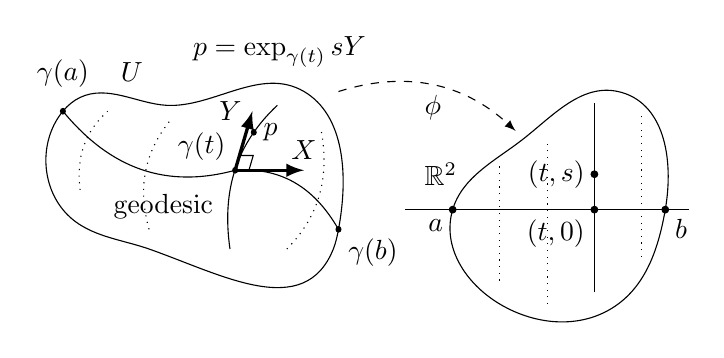
\begin{tikzpicture}
%uses hobby, calc library
    %here's the manifold
    \begin{scope}[xscale=0.875]
    
        %points \gamma(t), \gamma(a), \gamma(b)
	    \coordinate (O) at (0.5,0);
	    \coordinate (A) at (-2,0.75);
	    \coordinate (B) at (2,-0.75);
	    
	    %manifold blob
	    \path[draw,use Hobby shortcut,closed=true]
        (A) .. (-1.75,0.925) .. (-0.5,0.825) .. (1.5,1) .. (B) .. (1.925,-1) .. (-0.75,-1) .. (-2,-0.5);
        \draw (-1,1) node[anchor=south]{$U$};
	    
	    %hatchings
	    \draw[dotted]
	        (-1.75,-0.25) to[bend left] (-1.35,0.75);
	    \draw[dotted]
	        (-0.75,-0.75) to[bend left] (-0.45,0.625);
        \draw[]
	        (0.425,-1) to[bend left] coordinate[pos=0.775](P) ($(O)+(0.6125,0.825)$);
	    \draw[dotted]
	        (1.25,-1) to[bend right] (1.75,0.5);
        \filldraw (P) circle (1pt) node[anchor=west] {$p$};
	    
	    %unit vector pair
	    \draw[very thick, ->] (O)--(1.5,0) node[anchor=south] {$X$};
	    \draw[very thick, ->] (O)--($(O)+(0.25,0.75)$) node[anchor=east] {$Y$} coordinate[pos=0.25](ANG);
	    \draw
	        ($(O)+(0.2,0)$)--
	        ($(ANG)+(0.2,0)$)--
	        (ANG);
	    
	    %geodesic
	    \draw[] (A) to[bend right] node[pos=0.625, below=0.125cm]{geodesic} (O);
	    \draw[] (O) to[bend left] (B);
	    \filldraw[] (A) circle (1pt) node[above=0.5em] {$\gamma(a)$};
	    \filldraw[] (B) circle (1pt) node[anchor=north west] {$\gamma(b)$};
	    \filldraw[] (O) circle (1pt) node[anchor=south east] {$\gamma(t)$};    
    \end{scope}
    
    \draw (1,1.5) node {$p=\exp_{\gamma(t)}sY$};
    
    %mapping
    \draw[dashed, ->]
    (1.75,1) to[bend left] node[midway, below]{$\phi$} (4,0.5);
    
    %here's our coordinates
    \begin{scope}[shift={(5,-0.5)}, scale=0.6]
        %geodesic coordinates
        \coordinate (A) at  (-3,0);
        \coordinate (O) at   (0,0);
        \coordinate (B) at (1.5,0);
        
        %hatchings
        \draw[dotted] (-2,-1.5)--(-2,1);
        \draw[dotted] (-1,-2)--(-1,1.5);
        \draw[] (0,-1.75)--(0,2.25);
        \draw[dotted] (1,-1)--(1,2);
        
        \draw[]
            (-4,0) --
            (A) node[anchor=north east]{$a$} --
            (O) node[below left]{$(t,0)$} --
            (B) node[anchor=north west]{$b$} --
            (2,0);
            
        \filldraw (0,0.75) circle (2pt) node[left] {$(t,s)$};
        
        %euclidean blob
	    \path[draw,use Hobby shortcut,closed=true]
        (A) .. (-1.5,1.5) .. (0.5,2.5) .. (B) .. (0.5,-2) .. (-2,-2);
        \draw (-3.25,0.75) node {$\bR^2$};
        
        \foreach \i in {(A), (O), (B)}
        {
            \filldraw[] \i circle (2pt);
        }
    \end{scope}
\end{tikzpicture}
\end{document}